\documentclass[11pt,a4paper,oneside]{article}

\usepackage[T1]{fontenc}
\usepackage[polish]{babel}
\usepackage[utf8]{inputenc}
\usepackage{lmodern}
\usepackage{caption}
\usepackage{subcaption}
\usepackage{graphicx}
\usepackage{amsmath}
\usepackage{mathptmx}
\usepackage{float}
\usepackage{listings}
\usepackage[hidelinks]{hyperref}
\usepackage{mathtools}
\usepackage{titling}
\usepackage{tocloft}
\usepackage{xcolor}
\usepackage{lscape}
\usepackage{textcomp}
\usepackage{fancyhdr}
\usepackage{enumitem}
\usepackage{wrapfig}
\usepackage{siunitx,esvect}
\usepackage[a4paper,bindingoffset=0in,left=0.7in,right=0.7in,top=1in,bottom=1in,footskip=0.5in]{geometry}

\usepackage{tabularx}
\usepackage{booktabs}

\usepackage{realboxes}
\usepackage{xpatch}

\renewcommand{\cftsecleader}{\cftdotfill{\cftdotsep}} 

% Określamy nazwy 'table' oraz 'figure':
\AtBeginDocument{
  \renewcommand{\tablename}{Tabela}
  \renewcommand{\figurename}{Rys.}
}



\definecolor{lgray}{gray}{0.96}
\definecolor{lbcolor}{rgb}{0.9,0.9,0.9}
\lstset{
    framesep=2pt,
    basicstyle=\ttfamily,
    basicstyle=\small,
    aboveskip={0.75\baselineskip},
    columns=flexible,
    showstringspaces=false,
    frame=single,
    rulecolor=\color{lgray},
    showtabs=false,
    showspaces=false,
    showstringspaces=false,
    backgroundcolor=\color{lgray},
    identifierstyle=\ttfamily,
    keywordstyle=\color[rgb]{0,0,1},
    commentstyle=\color[rgb]{0.0,0.26,0.15},
    stringstyle=\color[rgb]{0.627,0.126,0.941}
}


\makeatletter
\xpretocmd\lstinline{\Colorbox{lgray}\bgroup\appto\lst@DeInit{\egroup}}{}{}
\makeatother

\setlength{\parskip}{1em}
\setlength{\parindent}{0pt}

\selectlanguage{polish}

\title{Algorytmy genetyczne - projekt} % The article title
\author{Arkadiusz Kasprzak\\Informatyka Stosowana\\Wydział Fizyki i Informatyki Stosowanej AGH} % The article author
\date{}

\pagestyle{plain} 

%%%%%%Strona tytulowa%%%%%
\begin {document}


\maketitle

\tableofcontents
\newpage

\pagestyle{fancy}
\fancyhf{}

\rhead{Arkadiusz Kasprzak}
\lhead{Algorytmy Genetyczne - projekt}
\cfoot{\thepage}

\section{Wstęp}
Wykonywany w ramach przedmiotu \textit{Algorytmy genetyczne} projekt zakładał stworzenie programu optymalizującego ułożenie zadanego zbioru prostokątnych płyt na obszarze o zadanym rozmiarze tak, by pozostało jak najmniej niezagospodarowanego miejsca. Do dyspozycji była zatem prostokątna płyta o wymiarach $2800 \times 2070~\si{mm}$ oraz zestaw maksymalnie 40 płyt do wycięcia z niej. Dozwolone były wyłącznie cięcia pionowe i poziomie, małe płyty nie mogły na siebie nachodzić lub wystawać poza dużą płytę. Przygotowane przeze mnie rozwiązanie oparte zostało o algorytm genetyczny wspomagany przez inne, pomniejsze algorytmy.

\section{Opis implementacji}
Program napisany został w języku C++ (z wykorzystaniem funkcjonalności standardu C++11 oraz C++14). Do jego implementacji wykorzystana została biblioteka GALib, w tym m.in. udostępniana przez nią możliwość tworzenia własnych typów stanowiących genomy. Ponadto przygotowane przez algorytm rozwiązanie może zostać ,,poprawione'' przez algorytm deterministyczny. W niniejszej części sprawozdania opisane zostaną kolejno elementy takie jak: przebieg działania programu, rodzaj zastosowanego algorytmu genetycznego czy zastosowane operatory: mutacji, selekcji i krzyżowania. Należy tutaj zwrócić uwagę, że bardzo często operatory oraz parametry algorytmu dobierane były metodą prób i błędów. Ze względu na ograniczoną objętość niniejszego sprawozdania opis tych badań został w wielu przypadkach pominięty.

\subsection{Działanie programu}
Działanie programu podzielić możemy na kilka etapów (rys. \ref{fig:fig1}):
\begin{itemize}[noitemsep, topsep=0pt]
\item inicjalizacja - wczytanie danych z pliku \textit{maleplyty.txt} oraz przygotowanie odpowiednich struktur, które te dane przechowują
\item wykonanie algorytmu genetycznego
\item sprawdzenie oraz ewentualna naprawa poprawności rozwiązania - na tym etapie program sprawdza, czy rozwiązanie jest poprawne. Jeśli któraś z płyt nie spełnia zadanych kryteriów, zostaje usunięta z rozwiązania.
\item próba poprawy rozwiązania - program dokonuje sprawdzenia, czy żadna z mniejszych płyt nie może zostać jeszcze dodana do już powstałego rozwiązania. Polega to po prostu na iteracji po współrzędnych dużej płyty i sprawdzaniu, czy w danym miejscu możliwe jest dodanie jeszcze jednej płyty - jeśli tak, jest ona dodawana. Algorytm ten jest bardzo prosty i pełni rolę wyłącznie wspomagającą. Nie wykonuje się, jeśli poprzednie etapy trwały dłużej niż 2 minuty.
\item zapis ostatecznego wyniku do pliku \textit{output.txt}
\end{itemize}

\begin{figure}[H]
\centering
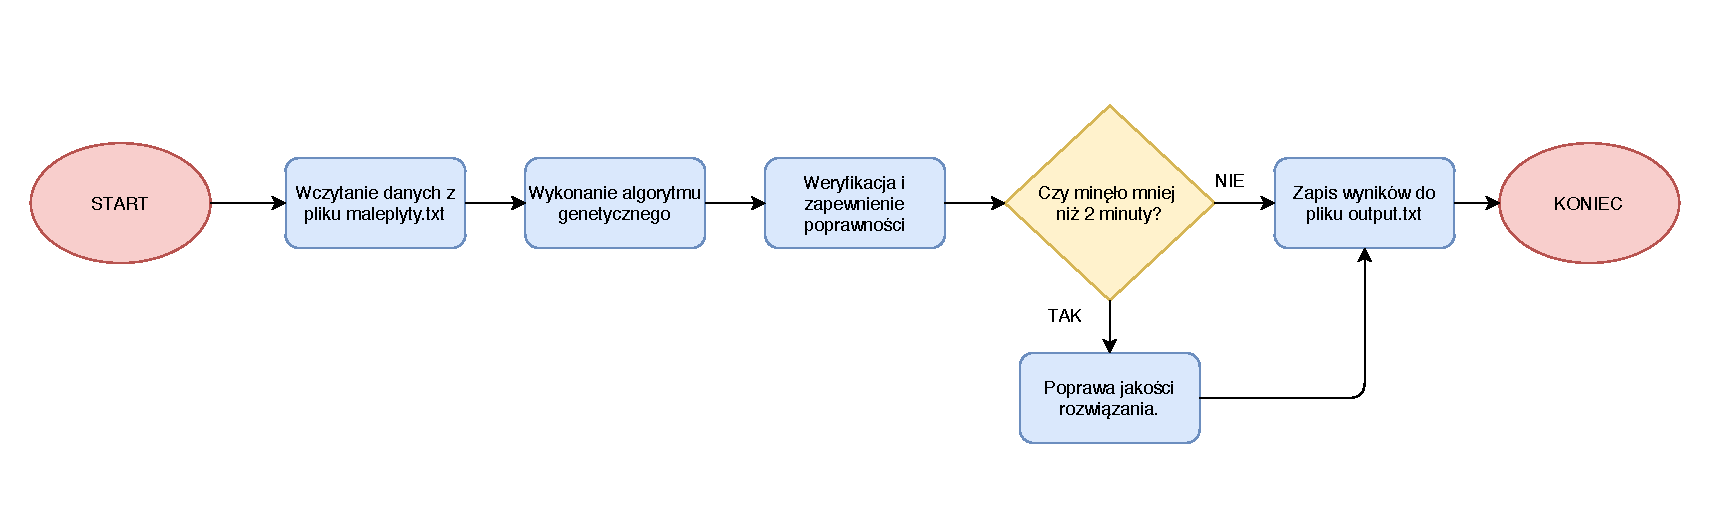
\includegraphics[width=0.82\textwidth]{res/Diagram.pdf}
\caption{Schemat blokowy ilustrujący działanie programu.}
\label{fig:fig1}
\end{figure}

\clearpage
\subsection{Zastosowany genom}
W programie zastosowany został stworzony przeze mnie na potrzeby algorytmu rodzaj genomu (jego implementację stanowi klasa \lstinline{CompositeGenome}). Składa się on z czterech genomów typu \lstinline{GA1DArrayAlleleGenome<int>} odpowiadających za przechowywanie w formie tablicy informacji o: współrzędnych x i y każdej z mniejszych płyt, fakcie, czy dana płyta została obrócona o 90 stopni oraz fakcie, czy dana płyta została w danym rozwiązaniu użyta. Każdy z genomów wyposażony jest w tzw. \lstinline{allele set}, określający możliwy zbiór wartości: w przypadku współrzędnych są to wymiary płyty, w pozostałych dwóch: wartości 0 i 1. Takie kodowanie daje stosunkowo dużą elastyczność w doborze operacji takich jak mutacja oraz sprawia, że każde z możliwych rozwiązań może być potencjalnie uwzględnione przez algorytm. Zastosowana została również bardzo specyficzna metoda inicjalizacji genomu: na początek genomy przechowujące położenia oraz rotację płyt zostają zainicjalizowane w sposób standardowy, za pomocą funkcjonalności \lstinline{allele set}. Genom przechowujący informację o tym, które płyty są wykorzystywane zainicjalizowany zostaje natomiast zerami. Następnie wybierana jest jedna z płyt, która zostaje umieszczona w punkcie $(0, 0)$ dużej płyty i dla niej wartość w genomie \lstinline{isUsed} zostaje ustawiona na 1. Taka procedura zwiększa prawdopodobieństwo, że stworzony genom będzie poprawny, a ponadto wymusza rozpoczęcie poszukiwań od rozwiązań wyrównanych do lewej i górnej krawędzi dużej płyty (znaczenie takiego postępowania zostanie szerzej opisane w dalszej części sprawozdania, dotyczącej mutacji).


\subsection{Zastosowany algorytm i jego parametry}
W programie zastosowany został algorytm typu \lstinline{GASteadyStateGA} z domyślną wartością parametru określającego ilość zastępowanych w każdym pokoleniu osobników. Algorytm ten w każdym pokoleniu tworzy populację składającą się z nowych osobników oraz osobników z poprzedniego pokolenia a następnie usuwa najgorsze osobniki tak, by populacja zachowała stały rozmiar. Zastosowanie tego algorytmu miało w przypadku mojego rozwiązania znaczny, pozytywny wpływ na uzyskane wyniki (względem domyślnego algorytmu \lstinline{GASimpleGA}). Ponadto metodą prób i błędów dobrane zostały następujące parametry: liczba pokoleń - 1000, wielkość populacji - 1000 osobników, prawdopodobieństwo mutacji - 0.05 (przy czym proces mutacji opisany poniżej uwzględnia nie tylko ten parametr) oraz prawdopodobieństwo krzyżowania - 0.75. Jakość działania algorytmu jest niestety w dużym stopniu zależna od wartości tych parametrów. W algorytmie zastosowany został dodatkowo niestandardowy mechanizm zakończenia algorytmu - kończy się on, jeśli udało się dotrzeć do ostatniego pokolenia lub jeśli minęło więcej niż 5 minut.


\subsection{Funkcja celu}
Zastosowana została bardzo prosta funkcja celu, wyliczająca pole wszystkich zastosowanych w rozwiązaniu figur i dzieląca je przez pole dużej płyty. Dla rozwiązań, które nie spełniają warunków zadania (zawierają nachodzące lub wystające płyty) przewidziana została wartość 0. Gwarantuje to, że z bardzo dużym prawdopodobieństwem wyprodukowane przez program rozwiązanie będzie poprawne. Testowana była ponadto metoda kar (zarówno w formie kwadratowej, jak i liniowej), natomiast jej stosowanie prowadziło do niebezpiecznych sytuacji, gdy np. w lewym górnym rogu dużej płyty jednocześnie znajdowały się dwie, zwykle znacznie różniące się rozmiarami, płyty. W tym przypadku metoda kar zdawała się nie przynosić tak dużych korzyści, jak inne zastosowane w algorytmie rozwiązania, została więc usunięta. Wyliczanie pola nakładających się figur wpływało ponadto negatywnie na wydajność algorytmu.

\clearpage
\subsection{Operator mutacji}
Najważniejszym elementem przygotowanego rozwiązania stanowi rozbudowany operator mutacji. Jego działanie opiera się na dwóch etapach:
\begin{itemize}[noitemsep, topsep=0pt]
\item zastosowanie standardowych metod mutacji: każda z płyt może zostać przesunięta o pewną niewielką liczbę w pionie oraz poziomie (stopień przesunięcia wyznaczany jest za pomocą rozkładu normalnego) z prawdopodobieństwem równym prawdopodobieństwu mutacji. Ponadto niezależnie od powyższego przesunięcia płyta może zostać obrócona lub dodana/usunięta z rozwiązania - w tym wypadu prawdopodobieństwo wynosi połowę prawdopodobieństwa mutacji. Każda z tych trzech operacji jest od siebie niezależna (wykonywane są trzy losowania), ponadto operacje na każdej z figur również są od siebie niezależne. Figura nie może zostać przesunięta tak, by jej położenie określały ujemne współrzędne, nie ma natomiast zabezpieczeń przed złamaniem pozostałych założeń zadania.
\item wyrównanie płyt w stronę osi układu współrzędnych z prawdopodobieństwem 0.25. W tym etapie płyty wyrównywane są najpierw w poziomie, a następnie w pionie. Dzięki temu promowane są rozwiązania, w których płyty przylegają do siebie. Ma to kluczowy wpływ na jakość otrzymywanych rozwiązań - zupełnie losowe rozłożenie płyt prowadziło do sytuacji, w których powstawało między nimi wolne miejsce. Było ono jednak za małe, by zmieściła się tam kolejna płyta, przez co pewna część przestrzeni była marnowana. Zastosowanie tej operacji w przypadku dostarczonego wraz z zadaniem zbioru testowego prowadziło do poprawy rozwiązania o około $800 000~\si{mm^2}$ (co stanowi około $15\%$ najlepszego uzyskanego rozwiązania, jest to zatem duży zysk). Efekt zastosowania tej operacji przedstawiony został na rysunku \ref{fig:fig2}.
\end{itemize}

\begin{figure}[H]
\begin{subfigure}{.49\textwidth}
    \centering
    
\includegraphics[width=.95\linewidth]{res/resultRaw.pdf}
    \caption{Brak algorytmu wyrównywania. Wynik: $4611959~\si{mm^2}$}
\end{subfigure}
\hfill
\begin{subfigure}{.49\textwidth}
    \centering
    
\includegraphics[width=.95\linewidth]{res/resultImp.pdf}
    \caption{Wykorzystanie algorytmu wyrównywania. Wynik: $5413959~\si{mm^2}$}
\end{subfigure}
\caption{Wyniki uzyskane bez oraz z użyciem algorytmu wyrównywania rozwiązania. Pominięte zostały algorytmy ulepszające rozwiązanie.}
\label{fig:fig2}
\end{figure}


\subsection{Operatory selekcji i krzyżowania}
W programie zastosowana została metoda selekcji ruletkowej. Odrzucone zostały: selekcja rankingowa (z powodu gorszych wyników oraz znacznego obniżenia wydajności) oraz turniejowa (z powodu gorszych wyników). Pozostałe metody nie były testowane. W algorytmie wyłączone zostało skalowanie. Zastosowany operator krzyżowania to krzyżowanie jednopunktowe - wykorzystana została tutaj po prostu procedura dostarczona przez bibliotekę GALib dla genomów typu \lstinline{GA1DArrayAlleleGenome<int>}. Nie były testowane inne operatory krzyżowania.

\section{Testy}
Przygotowane rozwiązanie poddane zostało przeze mnie testom - w tym celu wykorzystane zostały różne zbiory danych. Poniżej zamieszczam wyniki (w formie graficznej) dwóch przykładowych testów.

\begin{figure}[H]
\begin{subfigure}{.49\textwidth}
    \centering
    
\includegraphics[width=.95\linewidth]{res/result1.pdf}
    \caption{Konfiguracja podstawowa}
\end{subfigure}
\hfill
\begin{subfigure}{.49\textwidth}
    \centering
    
\includegraphics[width=.95\linewidth]{res/result2.pdf}
    \caption{Konfiguracja sześciu płyt o rozmiarach $1000 \times 2070~\si{mm}$.}
\end{subfigure}
\caption{Wyniki przykładowych testów}
\label{fig:fig3}
\end{figure}

Przetestowana została również odporność programu na sytuacje skrajne, takie jak: podanie dużej liczby płyt (sprawdzenie czasu zatrzymania) czy podanie takiego zestawu płyt, z których żadna nie mieści się na dużej płycie (sprawdzenie, czy program wybierze rozwiązanie poprawne, polegające na odrzuceniu każdej z płyt). Dla konfiguracji podstawowej (plik dostarczony wraz z treścią zadania) wynik zwykle nie jest niższy od $5000000~\si{mm^2}$.

\section{Podsumowanie}
W ramach projektu stworzony został program realizujący postawione założenia. Przygotowany algorytm mógłby prawdopodobnie zostać jeszcze dopracowany (np. poprzez dobór parametrów takich jak wielkość populacji) oraz zoptymalizowany. Planowane było rozwiązanie wielowątkowe, napotkane zostały jednak problemy natury technicznej (związane z biblioteką GALib). Sposób kodowania prawdopodobnie mógłby zostać uproszczony (z uwagi na fakt, że premiowane są wyrównane rozwiązania). Pomimo to algorytm produkuje rozwiązania do zadowalającej jakości.



\end {document}